\documentclass[11pt]{article}
\input{/Users/markwang/.preamble}
\begin{document}



% arg1=pdfurl arg2=pagenum arg3=sectiontitle
\newcommand{\linksection}[3][../../bishop_pattern_recognition_and_machine_learning.pdf]{
    \subsection*{\href[page=#2]{#1}{#3}}
}

\renewcommand{\norm}[1]{\left\lVert#1\right\rVert}
\renewcommand{\E}[2][]{\mathbb{E}_{#1}\left\{#2\right\}}
\newcommand{\var}[1]{var\{#1\}}
\newcommand{\cov}[1]{cov\{#1\}}
\newcommand{\normal}[1]{\mathcal{N}\left(#1\right)}
\newcommand{\exponents}[1]{exp\left\{#1\right\}}

\newcommand{\bmu}{\boldsymbol{\mu}}
\newcommand{\bphi}{\boldsymbol{\phi}}


\newcommand{\calR}{\mathcal{R}}
\newcommand{\calC}{\mathcal{C}}
\newcommand{\calD}{\mathcal{D}}
\newcommand{\bx}{\matr{x}}
\newcommand{\bX}{\matr{X}}
\newcommand{\bw}{\matr{w}}


\newcommand{\qqqquad}{\quad \quad \quad \quad}


\newcommand{\lebpar}[2]{\frac{\partial #1}{\partial #2}}
\newcommand{\balpha}{\boldsymbol{\alpha}}


\linksection{85}{Chapter 2 Probability Distribution}


\begin{defn*}
    \textbf{Introduction}
    \begin{enumerate}
        \item \textbf{Density Estimation} Model probability distribution $p(x)$ of a random variable $x$, given a finite set $x_1, \cdots, x_N$ of observations. 
        \item \textbf{Parametric Distribution} Probability distribution based on a fixed set of parameters. For example, Gaussian, binomial, multinomial are parametric distributions
        \item \textbf{Conjugate Priors} Priors that lead to posterior distribution having the same functional form (family) as the prior, and therefore lead to greatly simplified Bayesian analysis. THe conjugate prior for parameters of multinomial distribution is Dirichlet distribuution, while conjugate prior for Gaussian is another Gaussian. 
        \item \textbf{Nonparametric Distribution} Distribution which typically depends on size of data. For example, nearest-neighbours and kernels
    \end{enumerate}
\end{defn*}

\linksection{86}{2.1 Binary Variables}

\begin{defn*}
    \textbf{Bernoulli Variable} A single binary random variable $x\in \{0,1\}$ has Bernoulli distribution
    \[
        Bern(x|\mu) = \mu^x (1-\mu)^{1-x}   
    \]
    for $Bern(x|\mu)$, 
    \[
        \E{x} = \mu 
        \quad \quad 
        \var{x} = \mu(1-\mu)
    \]
    For $\mathcal{D} = \{x_1, \cdots, x_N\}$ where $x_i \overset{i.i.d.}{\sim} Bern(\mu)$
    \[
        p(\mathcal{D}|\mu)
        = \prod_{n=1}^N p(x_n | \mu)
        = \prod_{n=1}^N \mu^{x_n}(1-\mu)^{1-x_n}
    \] 
    \[
        \ln(p(\mathcal{D}|\mu))
        = \sum_{n=1}^N \ln{p(x_n|\mu)}
        = \sum_{n=1}^N \left(
            x_n\ln{\mu} + (1-x_n)\ln{(1-\mu)}
            \right)
    \]
    We obtain maximum likelihood estimator 
    \[
        \mu_{mle} = \frac{1}{N} \sum_{n=1}^N x_n    
    \]
    Note $m = \sum x_n$ is a sufficient statistics for Bernoulli distribution. 
\end{defn*}

\begin{defn*}
    \textbf{Binomial Distribution} Distribution of $m$ observations of $x=1$ given a data set size of $N$. We add a normalizing constant of $\binom{N}{m}$ representing all possible ways of obtaining $m$ distinct observations of $x=1$ where order does not matter
    \[
        Bin(m|N,\mu) = \binom{N}{m} \mu^m (1-\mu)^{N-m}
        \quad \quad \quad \quad 
        \binom{N}{m} = \frac{N!}{(N-m)!m!}
    \]
    For $Bin(m|N,\mu)$,
    \[
        \E{m} = \sum_{m=0}^N m Bin(m|N,\mu)= N\mu
        \quad \quad 
        \var{m} = \sum_{m=0}^N (m-\E{m})^2 Bin(m|N,\mu) = N\mu(1-\mu)
    \]
\end{defn*}

\begin{defn*}
    \textbf{Beta Distribution} as a conjugate prior of binomial distribution. We want to pick a distirbution such that the probability distribution is proportional to $\mu$ and $(1-\mu)$, the posterior distribution. Beta distribution is given by 
    \[
        Beta(\mu | a,b) = \frac{\Gamma(a+b)}{\Gamma(a)\Gamma(b)} \mu^{a-1}(1-\mu)^{b-1}
        \quad \quad \quad 
        \Gamma(x) = \int_0^{\infty} u^{x-1} e^{-u} du
    \]
    Note 
    \[
        \Gamma(x+1)=x\Gamma(x) \quad \quad \Gamma(x+1) = x!    
    \]
    The coefficients ensures that beta distribution is normalized such that it's a valid probability density function
    \[
        \int^1_0 Beta(\mu |a,b) d\mu = 1    
    \]
    The mean and variance given by 
    \[
        \E{\mu} = \frac{a}{a+b}
        \quad \quad \quad \quad 
        \var{\mu} = \frac{ab}{(a+b)^2(a+b+1)}
    \]
    We derive posterior distribution of $\mu$ by multiplying the beta prior with binomial likelihood 
    \begin{align*}
        p(\mu | m,l,a,b) 
        &\propto p(m|l,\mu)p(\mu|a,b) \\ 
        &=
        \binom{N}{m} \mu^m (1-\mu)^{N-m} \frac{\Gamma(a+b)}{\Gamma(a)\Gamma(b)} \mu^{a-1}(1-\mu)^{b-1} \\
        &\propto \frac{\Gamma(m+a+l+b)}{\Gamma(m+a)\Gamma(l+b)} \mu^{m+a-1} (1-\mu)^{l+b-1}
    \end{align*}
    where $l=N-m$, is number of observations where $x=0$. We see that $m$ observations of $x=1$ and $l$ observations of $x=0$ has been to increase value of $a$ by $m$ and $b$ by $l$. Hence, we can interpret $a$ and $b$ as effective number of observations of $x=1$ and $x=0$ respectively. Note the posterior distribution can act as the prior if we subsequently observe additional data.  \\
    \begin{center}
        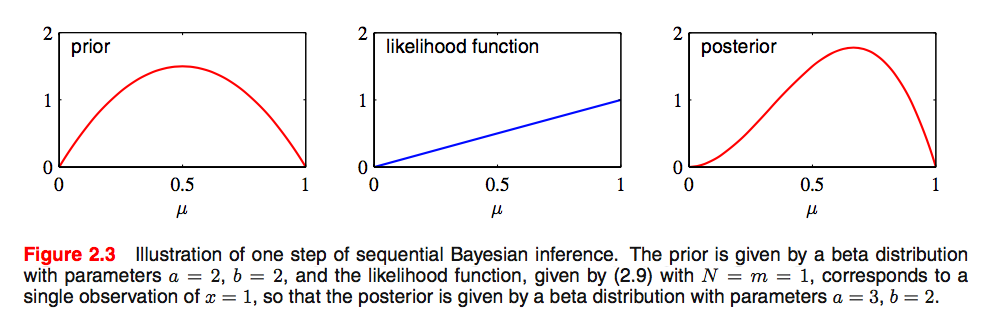
\includegraphics[width=12cm]{prior_to_posterior.jpg}
    \end{center}  
    The \textbf{sequential} approach to learning assumes i.i.d. data and used in real-tiome learning where a stream of data is arriving and that predictions must be made bfore all of the data is seen. Maximum likelihood can be cast into a sequential framework
\end{defn*}

\linksection{92}{2.2 Multinomial Variables}


\begin{defn*}
    \textbf{Multinomial Variables} A generalization of bernoulli variable, such that we have a discrete variable that can take on one of $K$ possible mutually exclusive states. One representation is 1-of-K scheme in which the variable is represented by a $K$-dimensional vector $\matr{x}$ in which one of $x_k = 1$ and all remaining elements equal 0, such that $\textstyle\sum_k x_k = 1$. We denote the probability of $x_k=1$ as $\mu_k$, then the distribution of $\matr{x}$ is given by 
    \[
        p(\matr{x}|\matr{\mu}) = \prod_{k=1}^K \mu_k^{x_k}
        \quad \quad \quad \quad 
        \matr{\mu} = (\mu_1,\cdots,\mu_K)^T 
        \quad 
        \mu_k \geq 0 \quad \textstyle\sum_k \mu_k = 1
    \]
    The distribution is a genearlization of Bernoulli distribution to more than two outcomes. Notice how the distribution is normalized 
    \[
        p(\matr{x}|\bmu) \geq 0
        \quad \quad \quad \quad 
        \sum_{\matr{x}} p(\matr{x}|\bmu) = \sum_{k=1}^K \mu_k^1 = 1
    \]
    \[
        \E{x|\mu} = \sum_{\matr{x}} p(\matr{x}|\bmu)\matr{x} = \sum_{k=1}^K \mu_k \matr{e}_k = (\mu_1, \cdots, \mu_M)^T = \bmu
    \]
    Assume a dataset of $N$ observations $\matr{x}_1,\cdots, \matr{x}_N$, the likelihood is given by 
    \[
        p(\mathcal{D}|\bmu) = \prod_{n=1}^N p(\matr{x}_n | \bmu)
        = \prod_{n=1}^N \prod_{k=1}^K \mu_k^{x_{nk}} 
        = \prod_{k=1}^K \mu_k^{(\sum_n x_{nk})} 
        = \prod_{k=1}^K \mu_k^{m_k}
        \quad\quad 
        \ln{p(\mathcal{D}|\bmu)} = \sum_{k=1}^K m_k \ln{\mu_k}
    \]
    where $m_k = \textstyle\sum_n x_{nk}$, a sufficient statistic representing the number of observations of $x_k =1$. We maximize $\ln{p(\mathcal{D}|\bmu)}$ with respect to $\mu_k$ taking account of the constraint the $\mu_k$ must sum to one with Lagrange multiplier. We maximize 
    \[
        \sum_{k=1}^K m_k \ln{\mu_k} + \lambda \left( \sum_{k=1}^K \mu_k - 1 \right)
    \]
    Setting derivative with respect to $\mu_k$ to zero, we have $\mu_k = - \rfrac{m_k}{\lambda}$. We solve for $\lambda$ with $\textstyle \sum_k \mu_k = 1$ gives $\lambda = -N$. We obtain maximum likelihood solution 
    \[
        \mu_k^{mle} = \frac{m_k}{N}    
    \]
    which is the fraction of $N$ observations for which $x_k =1$
\end{defn*}


\begin{defn*}
    \textbf{Multinomial Distribution} For n independent trials each of which leads to a success for exactly one of k categories, with each category having a given fixed success probability, the multinomial distribution gives the probability of any particular combination of numbers of successes for the various categories. The joint distribution of $m_1,\cdots, m_K$ conditioned on parameter $\bmu$ and on total number of $N$ observations is is known as multinomial distribution 
    \[
        Mult(m_1,m_2,\cdots, m_K | \matr{\mu}, N) = 
        \binom{N}{m_1 m_2 \cdots m_k} \prod_{k=1}^K \mu_k^{m_k}
    \]
    Multinomial distribution is a genearlization of binomial distribution. For example, it models the probability of counts for rolling a k-sided die n times. The normalization coefficients is the number of ways of partitioning $N$ objects into $K$ groups of size $m_1,\cdots, m_K$ and is given by 
    \[
        \binom{N}{m_1 m_2 \cdots m_k} = \frac{N!}{m_1!m_2!\cdots m_K!}
    \]
    with constraints $\textstyle \sum_k m_k = N$. 
    \[
        \E{x} = N \mu_k 
        \quad\quad 
        \var{x} = N\mu_k (1-\mu_k)    
        \quad\quad 
        \cov{m_j, m_k} = -N \mu_j \mu_k
    \]
\end{defn*} 


\begin{defn*}
    \textbf{Dirichelet Distribution} To find the conjugate prior for the parameter $\{\mu_k\}$ of the multinomial distribution, we see 
    \[
        p(\bmu | \boldsymbol{\alpha})
        \propto \prod_{k=1}^K \mu_k^{\alpha_k - 1}
        \quad \quad \quad \quad 
        0 \leq \mu_k \leq 1 \quad 
        \textstyle \sum_k \mu_k=1
    \]
    where $\balpha = (\alpha_1, \cdots, \alpha_K)^T$. The normalized form is called the Dirichlet distribution 
    \[
        Dir(\bmu | \balpha) = \frac{\Gamma(a_0)}{\Gamma(\alpha_1) \cdots \Gamma(\alpha_K)} \prod_{k=1}^K \mu_k^{\alpha_k - 1}
        \quad \quad \quad \quad 
        \alpha_0 = \sum_k \alpha_k
    \]
    Because of $\textstyle \sum_k \mu_k = 1$, the distribution over the space of $\{\mu_k\}$ is confined to a simplex of dimensionality $K-1$. For example, ofr $K=3$, we have \\
    \begin{center}
        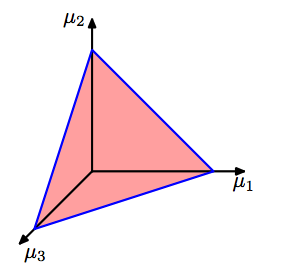
\includegraphics[width=5cm]{dirichlet_simplex.jpg}
    \end{center}
    To derive the posterior distribution, 
    \[
        p(\bmu|\mathcal{D}, \alpha) \propto p(\mathcal{D}|\bmu)p(\bmu|\balpha)
        \propto \prod_{k=1}^K \mu_k^{a_k+m_k-1}    
    \]
    which is also a Dirichlet distribution. Now we determine the normalization coefficients 
    \[
        p(\bmu|\mathcal{D},\balpha) = Dir(\bmu|\balpha + \matr{m}) 
        = \frac{\Gamma(\alpha_0 + N)}{\Gamma(\alpha_1 + m_1) \cdots \Gamma(\alpha_K + m_K)} \prod_{k=1}^K \mu_k^{\alpha_k + m_k - 1}
    \]
    where $\matr{m} = (m_1, \cdots, m_K)^T$ which are sufficient statistics from the dataset $\mathcal{D}$. We interpret $\alpha_k$ of Dirichilet prior as an effective number of observations of $x_k=1$ 
    \begin{center} 
        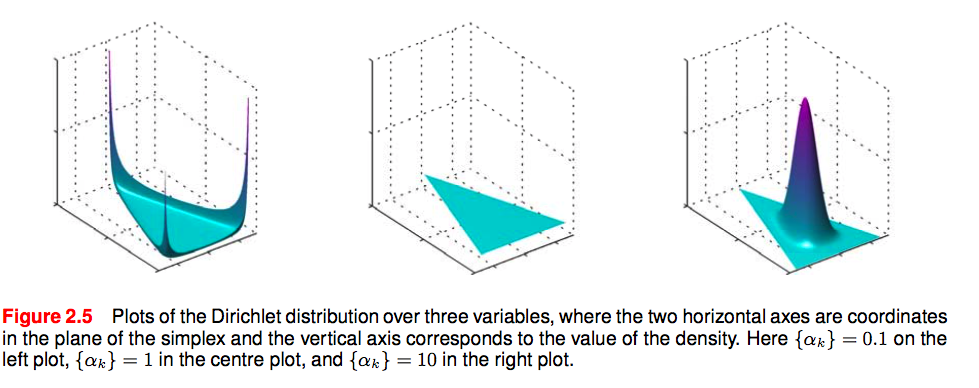
\includegraphics[width=10cm]{dirichlet.jpg}
    \end{center}
\end{defn*}

\linksection{96}{2.3 The Gaussian Distribution}

\begin{defn*}
    \textbf{Gaussian}
    \begin{enumerate}
        \item \textbf{Single Variable} 
        \[
            \normal{x|\mu, \sigma^2}
            = 
            \frac{1}{(2\pi \sigma^2)^{1/2}}
            \exponents{-\frac{1}{2\sigma^2}(x-\mu)^2}
        \]
        where $\mu$ is the mean, $\sigma^2$ is the variance
        \item \textbf{Multivariate}
        \[
            \normal{\matr{x|\boldsymbol{\mu}, \Sigma}}
            = 
            \frac{1}{(2\pi)^{D/2}}
            \frac{1}{|\matr{\Sigma}|^{1/2}}  
            \exponents{-\frac{1}{2} 
                \matr{(x-\bmu)^T \Sigma^{-1} (x-\bmu)}
            }
        \]
        where D-dimensional vector $\boldsymbol{\mu}$ is called the mean and $D\times D$ matrix $\matr{\Sigma}$ is the covariance matrix. 
        \item \textbf{Motivation} The central limit theorem states that the sum of a set of random variables, which in itself is a random variable, has a distribution that becomes increasingly Gaussian as the number of terms in the sum increases. 
        \item \textbf{Quadratic Form}
        \[
            \triangle^2 = (\matr{x} - \bmu)^T \matr{\Sigma}^{-1}(\matr{x} - \bmu)
        \]
        \item \textbf{Mahalanobis distance} The quantity $\triangle$ is called the Mahalanobis distance from $\mu$ to $\matr{x}$ and reduces to the Euclidean distance when $\matr{\Sigma}$ is the identity matrix. 
        \item \textbf{Covariance Matrix} can be expressed as 
        \[
            \matr{\Sigma} = \sum_{i=1}^D \lambda_i \matr{u}_i \matr{u}_i^T    
            \quad \quad \quad \quad 
            \matr{\Sigma}^{-1} =\sum_{i=1}^D \frac{1}{\lambda_i} \matr{u}_i \matr{u}_i^T
        \]
        where $\lambda_i$ and $u_i$ are eigenvalue and eigenvector of $ \matr{\Sigma}$. The quqdratic form can be written as 
        \[
            \triangle^2 = \sum_{i=1}^D \frac{y_i^2}{\lambda_i}   \quad \quad \quad \quad 
            y_i = \matr{u}_i^T (\matr{x-\bmu})
            \quad \quad 
            \matr{y = U(x-\bmu)}
        \]
        where $\{y_i\}$ can be interpreted as a new coordinate system defined by eigenvectors $u_i$. $\matr{U}$ is a matrix whose rows are given by $u_i^T$
        \begin{center}
            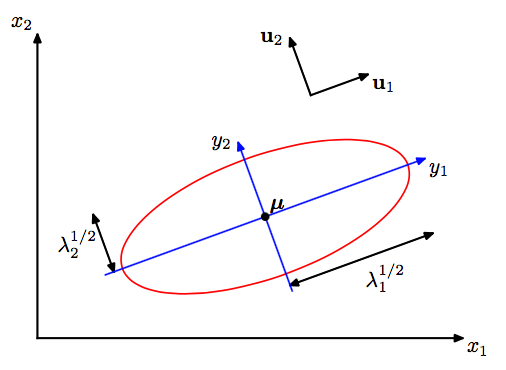
\includegraphics[width=5cm]{change_of_coord_gaussian.jpg}
        \end{center}
        For Gaussian distribution to be well defined, it is necessary and all of $\lambda_i$ are strictly positive, i.e. $\matr{\Sigma}$ is a positive definite matrix. For covariance matrix with some zero eigenvalues, distribution is singular and is confined to a subspace of lowe dimensionality. 
        \item \textbf{Expectation} given by 
        \[
            \E{x} = \bmu 
            \quad \quad 
            \cov{x} = \matr{\Sigma}
        \] 
        \item \textbf{Limitations} THe model parameter grows quadratically with $D$, computation task of inverting large matrices can become prohibitive. This can be alleviated by the use of isotropic covariance matrices $\matr{\Sigma} = \sigma^2 \matr{I}$, however restricts the ability to capture interesting correlations in the data. Another limitation is that it is unimodel (has a single maximum) so unable to model multimodal distributions. Introduction of latent variable solves these problems 
    \end{enumerate}
\end{defn*}

\linksection{111}{2.3.1 Conditional Gaussian Distribution}


\begin{defn*}
    \textbf{Conditional Gaussian Distribution} The conditional distribution of a set of Gaussian random variables conditioned on the another set is Gaussian. Similarly, the marginal distribution of either set is also Gaussian. Let $\matr{x} \sim \normal{\matr{x | \bmu, \Sigma}}$. We partition $\matr{x}$ into two sets such that 
    \[
        \matr{x} = 
        \begin{pmatrix}
            \matr{x}_a \\ \matr{x}_b
        \end{pmatrix}    
        \quad \quad \quad \quad 
        \matr{\mu} = 
        \begin{pmatrix}
            \matr{\mu}_a \\
            \matr{\mu}_b \\ 
        \end{pmatrix}
        \quad \quad \quad \quad 
        \matr{\Sigma} = 
        \begin{pmatrix}
            \matr{\Sigma}_{aa} & \matr{\Sigma}_{ab} \\
            \matr{\Sigma}_{ba} & \matr{\Sigma}_{bb} \\
        \end{pmatrix}
    \]
    where $\matr{x}_a$ and $\matr{x}_b$ has $M$ and $D-M$ components respectively. Define inverse of covariance matrix as the \textbf{precision matrix}
    \[
        \matr{\Lambda = \Sigma^{-1}}    
        \quad \quad \quad \quad 
        \matr{\Lambda} = 
        \begin{pmatrix}
            \matr{\Lambda}_{aa} & \matr{\Lambda}_{ab} \\
            \matr{\Lambda}_{ba} & \matr{\Lambda}_{bb}\\
        \end{pmatrix}
    \]
    Then condition distribution 
    \begin{align*}
        p(\matr{x}_a | \matr{x}_b) &= \normal{\matr{x}| \bmu_{a|b}, \Lambda_{aa}^{-1}} \\
        \bmu_{a|b} &= \bmu_a - \Lambda_{aa}^{-1} \Lambda_{ab} (\matr{x}_b - \bmu_b)
    \end{align*}
    and marginal distribution 
    \[
        p(\matr{x}_a) = \normal{\matr{x}_a | \bmu_a, \Sigma_{aa}}    
    \]
\end{defn*}


\linksection{111}{2.3.4 Maximum Likelihood for the Gaussian}

\begin{defn*}
    \textbf{Maximum Likelihood for the Gaussian} Given data set $\matr{X = (\bx_1, \cdots, \bx_N)^T}$ in which $\bx_n \overset{i.i.d.}{\sim} \normal{\matr{x}| \bmu, \matr{\Sigma}}$
    \[
        \ln{p(\matr{X}|\bmu, \matr{\Sigma})} = 
        = \frac{ND}{2} \ln{2\pi} - \frac{N}{2} \ln{|\matr{\Sigma}|} - \frac{1}{2} \sum_{n=1}^N (\bx_n - \bmu)^T \matr{\Sigma}^{-1}(\bx_n - \bmu)
    \]
    \[
        \frac{\partial}{\partial \bmu}  \ln{p(\matr{X}|\bmu, \matr{\Sigma})} = 
        \sum_{n=1}^N \matr{\Sigma}^{-1} (\bx_n - \bmu) = 0
        \quad \quad \rightarrow \quad \quad 
        \bmu_{mle} = \frac{1}{N}\sum_{n=1}^N \bx_n
    \]
    Note $\textstyle\sum_n x_n$ and $\textstyle \sum_n x_n x_n^T$ are sufficient statistics. Estimator for covariance matrix is given,
    \[
        \matr{\Sigma}_{mle} = \frac{1}{N}\sum_{n=1}^N (\bx_n - \bmu_{mle})(\bx_n - \bmu_{mle})^T
    \]
    We check to see if estimators are biased or not 
    \[
        \E{\bmu_{mle}} = \bmu \text{ (unbiased)}
        \quad \quad \quad \quad 
        \E{\matr{\Sigma}_{mle}} = \frac{N-1}{N} \matr{\Sigma} \text{ (biased)}
    \]
\end{defn*}


\linksection{112}{2.3.5 Sequential Estimation}


\begin{defn*}
    \textbf{Points}
    \begin{enumerate}
        \item \textbf{Sequential Estimation} for Gaussian Mean 
        \[
            \bmu_{mle}^{(N)} = \bmu_{mle}^{(N-1)} + \frac{1}{N} (\bx_N - \bmu_{mle}^{(N-1)})
        \]
    \end{enumerate}
\end{defn*}


\linksection{120}{2.3.7 Student's t-distribution}

\begin{defn*}
    \textbf{Student's t} Univariarnt Gaussian with Gamma prior, then integrate out precision, resulting in marginal distribution of $x$
\end{defn*}


\linksection{128}{2.3.9 Mixture of Gaussian}


\begin{defn*}
    \textbf{Points}
    \begin{enumerate}
        \item \textbf{Mixture of Gaussian} Linear combination of Gaussians gives better characterization of data
        \[
            p(\bx) = \sum_{k=1}^K \pi_k \normal{\bx|\bmu_k, \matr{\Sigma}_k}    
            \qquad 
            \sum_{k=1}^K \pi_k = 1
            \quad 
            \pi_k \geq 0
        \]
        Log maximimum likelihood for $\boldsymbol{\pi}, \bmu, \matr{\Sigma}$ has no closed solution
        \[
            \ln{p(\matr{X}| \matr{\boldsymbol{\pi}, \bmu, \Sigma})} = 
            \sum_{n=1}^N \ln{\sum_{k=1}^K \boldsymbol{\pi}_k \normal{\bx_n | \bmu_k , \matr{\Sigma}_k}}
        \]
    \end{enumerate}
\end{defn*}

\linksection{130}{2.4 The Exponential Family}

\begin{defn*}
    \textbf{Points}
    \begin{enumerate}
        \item Exponential Family over $\bx$, given parameters $\boldsymbol{\eta}$ is defined to be the set of distribution with form 
        \[
            p(\bx | \boldsymbol{\eta})
            = h(\bx) g(\boldsymbol{\eta}) \exponents{\boldsymbol{\eta}^T \matr{u(x)}}    
        \]
        where $\matr{u}$ is a function of $\bx$, $\boldsymbol{\eta}$ are natural parameters. $g(\boldsymbol{\eta})$ is the coefficients that ensures the distribution is normalized 
        \[
            g(\boldsymbol{\eta}) \int h(\bx) \exponents{\boldsymbol{\eta}^T \matr{u}(\bx)} d\matr{x} = 1
        \]
        \item bernoulli distribution 
        \item multinomial distribution
        \item MLE for Exponential Family 
        \[
            -\nabla \ln{g(\boldsymbol{\eta})} = \E{\matr{u(x)}}
        \]
        for which we can solve for $\boldsymbol{\eta}$ given only sufficient statistics $\matr{u(x)}$
        \[
            -\nabla \ln{g(\boldsymbol{\eta}_{mle})} = \frac{1}{N} \sum_{n=1}^N \matr{u(x)_n}
        \]
    \end{enumerate}
\end{defn*}




\end{document}
